\chapter{Introduction}

\section{Motivation}
The medical discipline of pathology is in a digital transformation. Instead of looking at tissue samples through the means of traditional light microscopy, it is now possible to digitize those samples. This digitalization is done with the help of a so called slide scanner. The result of such an operation is a \emph{whole slide image} (WSI)\nmc{WSI}{Whole Slide Image}\cite{Cornish13}. The digital nature of WSIs opens the door to the realm of image processesing and analysis which yields certain benefits, such as the use of image segmentation and registration methods to support the pathologist in his/her work.

A very promising approach to image analysis is the use of \emph{neural networks}\footnote{See chapter 2.2}\nmc{NN}{Neural Network}. These are a group of computational models inspired by our current understanding of biological NN. The construct of many interconnected neurons is considered a NN (both in the biological and artificial context). Each single one of those neurons has input values and an output value. Once the input reaches a certain trigger point, the cell in the neuron sends a signal as output. The connections between the neurons are weighted and can dampen or strengthen a signal. Because of this, old pathways can be blocked and new ones created. In other words, a NN is capable of "learning"\cite{Kriesel07}. This is a huge advantage compared to other software models. While certain problems are "easier" to solve in a sequential, algorithmic fashion (say an equation or the towers of hanoi), certain problems (e.g. image segmentation or object recognition) are very complex, so that new approaches are needed, while other problems can't be solved algorithmically at all. With the use of adequate training samples, a NN can learn to solve a problem, much like a human.

\begin{figure}[ht]
	\begin{center}
		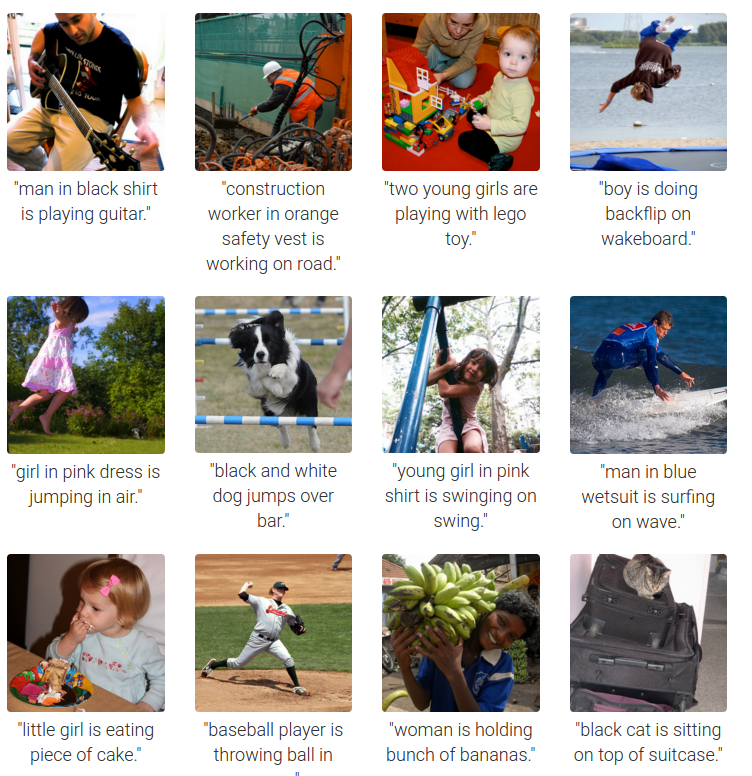
\includegraphics[scale=0.3]{img/deepVisual.png}
		\caption{Example results of the in \cite{Karpathy15} introduced model (source: \url{http://cs.stanford.edu/people/karpathy/deepimagesent/})}
		\label{fig:fig1.1}
	\end{center}
\end{figure}

In the recent past the use of NN enabled major breakthroughs, especially in the area of image classification and object recognition. Karpathy and Fei-Fei, for example, created a NN that is capable of describing an image or a scene using natural language text blocks \cite{Karpathy15} (see fig. 1.1 for a selection of examples).

There is enormous potential in the use of NN in the digital pathology as well, but to transfer these models and technologies, certain obstacles must be overcome. One of those is the need for proper training samples. While generally there are large amounts of WSIs (e.g. publicly available at the Cancer Genome Atlas\footnote{\url{https://gdc-portal.nci.nih.gov/}}), most of them won't be usable as a training sample without further preparation.

A possible way to prepare them is by using image annotation: tagging regions of interest (ROI)\nmc{ROI}{Regions of Interest} on an image and assigning labels or keywords as metadata to those tags. These can be added to the WSIs, stored and later used for training. The result of such an approach could be similar to the one of Karpathy and Fei-Fei\cite{Karpathy15}, but with a medical context instead of daily situations.

Therefore the goal of this thesis is to provide tools for pathologists and data scientists to annotate WSIs and save those annotations in such a way that they will be usable later in combination with NN.


\section{Research Objective}
The objective of this thesis is the conceptualization and implementation of tools to prepare WSIs for the further use as training samples in NN. To achieve this, a process chain with all the necessary steps needs to be established. The chain consists of the following tasks:
\begin{enumerate}[(A)]
	\item open WSI with a viewer tool
	\item annotate opened WSI
	\item extract annotations and prepare them for the use as training sample in a NN
\end{enumerate}

There is no standardized WSI file format\cite{Cornish13}. Hence, slide scanner vendors developed their own proprietary solutions. This either leads to
\begin{enumerate}[(i)]
	\item locking-in on a specific vendor or
	\item separate handling of each proprietary format
\end{enumerate}
(i) would render the whole process chain vendor specific, limiting it's use drastically. (ii) would not render the process chain vendor specific but call for a lot of additional work and maintenance, due to the separate handling of different formats. To counteract this, open file formats have been specified\cite{Cornish13}:
\begin{itemize}
	\item JPEG2000
	\item TIFF
	\item Deep Zoom Images (DZI)\nmc{DZI}{Deep Zoom Images}
	\item DICOM (supplement 145), without reference implementation as of yet\cite{Cornish13}
\end{itemize}
Therefore, to achieve (A), the first step of the process chain is to establish a tool with which WSIs of various vendor specific formats can be turned into an open file format. This way, neither (i) nor (ii) will arise as a problem.

To achieve (A) and (B), it is also necessary to deploy a graphical user interface (GUI)\nmc{GUI}{Graphical User Interface}, that not only makes it possible to open and view a WSI (A), but also enables the user to annotate the WSI, as well as manage made annotations (B).

To achieve (C), another tool needs to be established, that is capable of turning saved annotations into training samples which are prepared for a further use in NN.

In summary: to reach the research objective of this thesis, tools to achieve the following tasks need to be established:
\begin{enumerate}[(a)]
	\item conversion of various WSI formats into an open format
	\item annotation of WSIs and management thereof
	\item extracting and preparing annotations as training samples for later use in NN
\end{enumerate}

\section{About this thesis}
This thesis contains 6 chapters.

\emph{Chapter 1 - Introduction} and \emph{2 - Background} address the scope, background and vocabulary of this thesis.

The chapters 3 to 5 address the components described in the last section: \emph{chapter 3 - Conversion Service} will describe a tool for image conversion, \emph{chapter 4 - Annotation Service} will describe a tool for image annotation and \emph{chapter 5 - Tessellation Service} will describe an extraction tool, to prepare the annotations made with the Annotation Service for the use in a NN.

Finally, \emph{Chapter 6 - Conclusion} will discuss and conclude the findings of the aforementioned chapters.